\documentclass[10pt,twocolumn]{article}
\usepackage{times}
\usepackage{multirow}
\usepackage{subcaption}
\usepackage{graphicx,grffile}
\usepackage{pgf}
\usepackage{tikz}
\usetikzlibrary{arrows,automata}
\usepackage[latin1]{inputenc}

% do not change these values
\baselineskip 12pt
\textheight 9in
\textwidth 6.5in
\oddsidemargin 0in
\topmargin 0in
\headheight 0in
\headsep 0in

%\makeatletter
%\def\maxwidth{\ifdim\Gin@nat@width>\linewidth\linewidth\else\Gin@nat@width\fi}
%\def\maxheight{\ifdim\Gin@nat@height>\textheight\textheight\else\Gin@nat@height\fi}
%\makeatother
%% Scale images if necessary, so that they will not overflow the page
%% margins by default, and it is still possible to overwrite the defaults
%% using explicit options in \includegraphics[width, height, ...]{}
%\setkeys{Gin}{width=\maxwidth,height=\maxheight,keepaspectratio}
%

\usepackage[unicode=true]{hyperref}
\hypersetup{breaklinks=true,
            bookmarks=true,
            pdfauthor={},
            pdftitle={},
            colorlinks=true,
            citecolor=blue,
            urlcolor=blue,
            linkcolor=blue,
            pdfborder={0 0 0}}
\urlstyle{same}  % don't use monospace font for urls

\usepackage[font=footnotesize,labelfont=bf]{caption}

\begin{document}

\title{outline!}

\author{
%Noah Watkins, Neha Ojha\textsuperscript{*}, Carlos Maltzahn \\
%\small {\em University of California, Santa Cruz} \\
%\small {\{jayhawk,carlosm\}@cs.ucsc.edu} \textsuperscript{*}nojha@ucsc.edu \\ [2mm]
\small Submission Type: Research
}

\date{}
\maketitle

\begin{abstract}
\end{abstract}

\section{Introduction}

Cloud providers are increasingly reliant upon application-specific extensions
to distributed storage system such as Ceph as is shown in
Figure~\ref{fig:objclass-dev} by a marked increase in Ceph extensions used in
production.

The construction of extensions is not limited to core developers; the
development community has been receptive to contributions with the recent
inclusion by CERN developers of an extension for performing limited numeric
operations on object data~\cite{cls_numops}.

This trend is also not limited to Ceph. AWS Lambda, Redis Lua, Redis Modules,
KV-Drives, and Rhea, are all recent examples of storage systems embracing the
power of including application-specific semantics. While Ceph has not yet
reached the point of directly exposing these features to users, the recent
inclusion of a mechanism for dynamically defining extensions using
Lua~\cite{cls_lua} suggests that aspects of this may soon appear.

If the growth illustrated in Figure~\ref{fig:objclass-dev} continues, the
amount of low-level C++ will grow large. Unfortunately, much of
this code is written assuming a performance profile defined by a combination
of the hardware and software versions available at the time of development. As
Ceph development continues at a fast pace, the cost of adapting to changing
assumptions regarding performance will become significant.

% footnote: we could probably look through the cls_* changelog and find
% examples of changes based on changes to semantics.

% Virtualization. Operating systems and containers are similar. AUFS, dockerfile

Previous work in active storage has focused on the utility of moving
computation closer to data in an effort to reduce data movement and take
advantage of cpu and i/o parallelism, and gave little to no attention to
security or performance isolation concerns. In contrast, the interfaces being
deployed today focus on data management, indexing, and physical format.

\begin{figure}[ht]
  \centering
    \includegraphics[width=0.48\textwidth]{experiments/objclass-dev/output.png}
    \caption{
[\href{https://github.com/noahdesu/zlog-popper/tree/master/experiments/objclass-dev/visualize.ipynb}{source}]
Growth of officially supported, custom object interfaces in RADOS over 6
years. A \emph{method} is a specific object interface and a \emph{class} is a
logical grouping of methods.
}
\label{fig:objclass-dev}
\end{figure}

We propose the introduction of a declarative language for building object
based interfaces that allows a storage system to meet the needs of an
application throughout the development process without requiring rewrites.

\section{Background}

In this section we briefly describe Ceph and object-based interface
development. We will use CORFU as a motivating example of an interface, and
then show the challenges with the current low-level mechanisms for defining
interfaces.

\subsection{Domain-specific Object Interfaces}

Ceph allows the construction of domain specific interfaces. There are many
different object interfaces in production today. An example of the spectrum of
interface types is shown in Table~\ref{tab:objclass-cats}. Object classes are
developed as a transactional composition of native storage interfaces.

\begin{table}
\begin{tabular}{|l|l|l|}
\hline
Category & Specialization & Methods \\ \hline
\multirow{2}{*}{Locking} & Shared & \multirow{2}{*}{6} \\
                         & Exclusive & \\ \hline
\multirow{3}{*}{Logging} & Replica & 3 \\
                         & State & 4 \\
                         & Timestamped & 4 \\ \hline
GC & Reference Counting & 4 \\ \hline
\multirow{4}{*}{Metadata} & RBD & 37 \\
 & RGW & 27 \\
 & User & 5 \\
 & Version & 5 \\ \hline
\end{tabular}
\caption{A variety of RADOS object storage classes exist that expose reusable
interfaces to applications.}
\label{tab:objclass-cats}
\end{table}

\subsection{Motivating Example: CORFU}

The primary motivating example we will use in this paper is the CORFU
distributed shared-log designed to provide high-performance serialization
across a set of flash storage devices~\cite{balakrishnan:nsdi12}. The
shared-log is a powerful abstraction useful when building distributed systems
and applications, but common implementations such as Paxos or Raft funnel I/O
through a single node limiting the throughput of log
operations~\cite{lamport:tocs89}. The CORFU protocol addresses this limitation
by de-coupling log entry storage from log metadata, making use of a
centeralized, volatile, in-memory \emph{sequencer service} that assigns log
positions to clients that are appending to the log. Since the sequencer is
centeralized serialization is trivial, and the use of non-durable state allows
the sequencer service to operate at very high rates.

While a full description of the CORFU protocol is beyond the scope of this
paper, it is important to highlight the usage of application-specific flash
I/O interfaces in CORFU that are used to guarantee correctness during failure.
Each flash device in CORFU exposes a 64-bit write-once address space
consisting of the primary interfaces \emph{write(pos, data)} and
\emph{read(pos)}, as well as \emph{fill(pos)} and \emph{trim(pos)} that
invalidate and reclaim log entries, respectively. All I/O operations initiated
by clients are tagged with an \emph{epoch} value, and flash devices are
expected to reject client requests requests tagged with an old epoch value. To
facilitate recovery or handle system reconfiguration in CORFU, the storage
devices are also required to support a \emph{seal(epoch)} command that marks
the latest epoch and returns the maximum position written to that device. The
seal interface is used following the failure of a sequencer to calculate the
tail of the log that the sequencer should use to repopulate its in-memory
state.

\paragraph*{Programmable Storage and CORFU}
Two aspects of CORFU make its design attractive in the context of
the Ceph storage system. First, CORFU assumes a cluster of flash devices
because log-centric systems tend to have a larger percentage of random reads
making it difficult to achieve high-performance with spinning disks. However,
the speed of the underlying storage does not affect correctness. Thus, in a
software-defined storage system such as Ceph a single implementation can
transparently take advantage of any software or hardware upgrades, and make
use of data management features such as tiering in RADOS, allowing users to
freely choose between media types such as SSD, spinning disks, or emerging
NVRAM technologies.

The second property of CORFU relevant in the context of Ceph is the dependency
CORFU places on the storage device interface.  As was previously discussed, in
order to enforce constraints defined within the CORFU protocol, storage
devices are expected to expose a domain-specific interface specially designed
for the protocol. While the authors of the CORFU paper describe both a
host-based and FPGA-based solution, RADOS directly supports the concept of
custom storage interfaces to its objects that can be used to achieve the
transactional semantics necessary to implement the CORFU storage interfaces.
This feature is called RADOS object classes, and is one of the most powerful
features offered by RADOS for designing storage applications.

\paragraph*{A CORFU Object Interface}
The state-machine shown in Figure~\ref{fig:corfu-sm} shows the composition of
actions for each component of the CORFU interface. For example, each
operations begins with an \emph{epoch guard}, and a \emph{write} operation
will consult an index and perform a bulk I/O operation.  The primary concern
when mapping an interface onto Ceph is deciding how each native interface is
used in the interface composition.

\begin{figure}
\centering
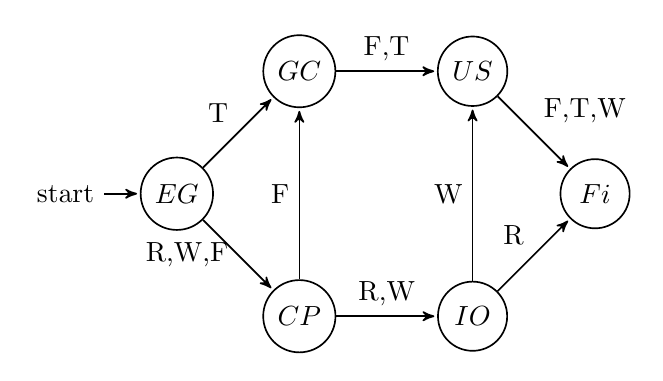
\begin{tikzpicture}[->,>=stealth',shorten >=1pt,auto,node distance=2.2cm,semithick]
%\tikzstyle{every state}=[fill=red,draw=none,text=white]

  \node[initial left,state] (A)              {$EG$};
  \node[state]         (B) [below right of=A] {$CP$};
  \node[state]         (D) [right of=B]       {$IO$};
  \node[state]         (C) [above right of=A] {$GC$};
  \node[state]         (E) [right of=C]       {$US$};
  \node[state]         (F) [below right of=E] {$Fi$};

  \path (A) edge        node [left] {R,W,F} (B)
            edge        node {T}     (C)
        (B) edge        node {F}     (C)
            edge        node {R,W}   (D)
        (C) edge        node {F,T}   (E)
        (D) edge        node {W}     (E)
            edge        node {R}     (F)
        (E) edge        node {F,T,W} (F);
\end{tikzpicture}
\caption{State transition diagram for read ($R$), write ($W$), fill ($F$), and
trim ($T$) CORFU operaitons. The states epoch guard ($EG$), check position ($CP$),
and update state ($US$) access metadata. The I/O performs a log entry read or
write, and garbage collection ($GC$) marks entries for reclamation.}
\label{fig:corfu-sm}
\end{figure}

\subsection{Physical Design}

There is a finite set of strategies for mapping the CORFU interfaces onto the
current set of native I/O interfaces used to construct object interfaces.
Table~\ref{tab:pd-map} shows the design space for mapping the CORFU interfaces
onto Ceph. In order to select the best mapping we performed a parameter sweet
over the design space.

\begin{figure*}[!ht]
    \centering
    \begin{subfigure}{.6\columnwidth}
        \includegraphics[width=\columnwidth]{experiments/librados-sweep/output.soft.reset.2hr.png}
        \caption{a}
        \label{fig:vanilla-io-diff}
    \end{subfigure}\hfill
    \begin{subfigure}{.6\columnwidth}
        \includegraphics[width=\columnwidth]{experiments/basic-cls-rand-read/output.read.60min.png}
        \caption{b}
    \end{subfigure}\hfill
    \begin{subfigure}{.6\columnwidth}
        \includegraphics[width=\columnwidth]{experiments/basic-cls-overhead/output.1024.soft.reset.png}
        \caption{c}
    \end{subfigure}\hfill
    \caption{Shown here are the graphs and such that demonstrate that the same
        physical design choices are not the same between differing version of
    Ceph even on the same hardware.}
\end{figure*}

Figure~\ref{fig:vanilla-io-diff} shows the result of a parameter sweep which
clearly shows that an N-1 mapping based on the bytestream interface provides
superiour performance. However, the other two graphs show the same interfaces
running on an old version of Ceph that show the same decision would not have
been the optimal choice {\bf \emph{note: for the outline these are not the
real graphs we'll be using}}.

\begin{table}
\begin{tabular}{ | l | l | l | l | l |}
\hline
Map & I/O & Entry Size & Addressing & Metadata \\ \hline
\multirow{3}{*}{1:1} & KV  & Flex     & Ceph      & KV/BS \\ \cline{2-5}
                     & BS  & Flex     & Ceph/VFS  & KV/BS \\ \hline
\multirow{4}{*}{N:1} & KV  & Flex     & \multicolumn{2}{|c|}{KV/BS} \\ \cline{2-5}
                     & WR  & Fixed    & VFS       & KV/BS \\ \cline{2-5}
                     & AP  & Flex     & KV/BS     & KV/BS \\
\hline
\end{tabular}
\caption{The high-level design space of mapping CORFU log entry storage onto
the RADOS object storage system.}
\label{tab:pd-map}
\end{table}

\section{Programming Model}

In this section we are going to be describing our way of creating interfaces.

\section{Other Interfaces}

Here we show the derivation of two other interfaces that are in production in
Ceph today to demonstrate the generality of our interface.

\section{Evaluation}

\section{Related Work}

\section{Conclusion}

%In this section we examine the design space for implementing the CORFU
%protocol in the RADOS storage system. Table \ref{t:init-ds} shows the entire
%design space. A description of each design parameter follows:
%
%{\bf Mapping strategy.} The method by which a log entry---identified by its
%logical position---is addressed within RADOS is referred to as the mapping
%strategy. A 1:1 strategy stores each log entry in a RADOS object with a
%distinct name (e.g. ``mylog.pos443''), and an N:1 strategy stripes the log
%positions across a set of objects (e.g.  round-robin). While we do consider
%both strategies in this paper, a 1:1 strategy is attractive because it allows
%a design in which clients can directly address log positions by constructing
%the correct object name.
%
%{\bf Storage interface.} entry data may be small or large. its primary
%storage location is important. kv, bs. we further sub-divide bs into
%write and append. each strategy is compatible with fixed size entries
%except for the write interface.
%
%{\bf Logical addressing.}

%\subsection{Storage Interface Selection}
%
%Figure \ref{f:librados-sweep} shows the single-node write-only I/O throughput
%for each of the points in the design space defined in Table \ref{t:init-ds}.
%The results reveal poor relative performance using both the key-value storage
%interface, as well as either of the 1:1 strategies---which incur overhead by
%creating a new object for each log entry. Both of the N:1 strategies using the
%bytestream I/O interface outperform all of the other approaches by over 2x
%throughput, but otherwise have nearly identical performance.
%
%To examine the read performance of the points in the design space we generated
%a dataset using each of the write workloads, and then issued random reads
%across the entire dataset. Figure \ref{f:librados-rand-read} shows the read
%throughput for each of the design strategies. The results show that an N:1
%mapping using bytestream interface performs best. Interestingly, the 1:1
%mapping strategy using the bytestream interface exhibits good read performance
%in comparison to writes using the same strategy.

%\begin{figure}[h]
%  \centering
%  \includegraphics[width=0.45\textwidth]{experiments/librados-sweep/output.soft.reset.2hr.png}
%  \caption{
%[\href{https://github.com/noahdesu/zlog-popper/tree/master/experiments/librados-sweep/visualize.ipynb}{source}]
%Throughput (IOPS) of 1K writes to a single OSD using the standard I/O
%interfaces in various configurations. The best performance is achieved using
%the byte stream interface and a N:1 mapping strategy.
%}
%\end{figure}
%
%\begin{figure}[h]
%  \centering
%  \includegraphics[width=0.45\textwidth]{experiments/basic-cls-rand-read/output.read.60min.png}
%  \caption{
%[\href{https://github.com/noahdesu/zlog-popper/tree/master/experiments/basic-cls-rand-read/visualize.ipynb}{source}]
%Throughput of 1K random reads to a single OSD using the standard I/O
%interfaces in various configurations. The best performance is achieved using
%the byte stream interface and a N:1 mapping strategy.
%}
%\end{figure}
%
%\begin{figure}[h]
%  \centering
%  \includegraphics[width=0.45\textwidth]{experiments/basic-cls-overhead/output.1024.soft.reset.png}
%  \caption{
%[\href{https://github.com/noahdesu/zlog-popper/tree/master/experiments/basic-cls-overhead/visualize.ipynb}{source}]
%}
%\end{figure}


%As a first approximation these results show that when optimizing for log
%append and random read throughput the design space should be refined by
%limiting solutions to architectures based on a N:1 mapping strategy using the
%bytestream I/O interface. But what these microbenchmarks explicitly omit are
%the overheads associated with metadata management such as enforcing write-once
%semantics or using an index to map a log position to a physical offset within
%an object. In the next section we

\bibliography{paper}
\bibliographystyle{plain}

\end{document}
